% IISE DAIS Best Student Paper Competition - Main Content
% Shared by both blinded and unblinded versions

% Abstract
\begin{center}
\textbf{\fontsize{12}{14}\selectfont Abstract}
\end{center}

\noindent
Large Language Models enable modern AI applications but incur high costs—ChatGPT's daily inference exceeds \$700,000. We develop threshold-based scheduling algorithms for LLM inference under memory constraints. Dynamic Key-Value cache growth creates eviction risks that degrade throughput by 12-25\% even when capacity is sufficient. Using fluid dynamics from queueing theory, we characterize equilibrium where arrivals match completions, revealing optimal memory $M^*$. Our algorithms—WAIT (known output lengths) and Nested WAIT (unknown outputs)—maintain systems near equilibrium through controlled admission. Nested WAIT uses on-the-fly classification: short prompts complete early while long prompts advance to later segments, eliminating output prediction. Validation on real-world LMSYS-Chat-1M data and NVIDIA A100 GPUs achieves 12-25\% throughput improvement over vLLM and Sarathi.

% Keywords
\textbf{\fontsize{12}{14}\selectfont Keywords}

\noindent
LLM inference, online scheduling, memory constraints, queueing theory, throughput optimization

% Main content sections
\section{Introduction}

LLMs power chatbots, search, and programming assistants \cite{brown2020language,openai2024gpt4technicalreport}, generating extensive operational data (arrival rates, prompt lengths, latency) that inform scheduling \cite{strubell2019energy}. LLM inference has two phases: \textit{prefill} (process input) and \textit{decode} (generate output). The Key-Value cache stores representations but consumes GPU memory growing linearly with output length. Batching improves throughput but risks exceeding capacity $C$, forcing \textit{eviction}—restarting prompts and wasting computation.

\textbf{Eviction Challenge.} Memory sufficiency doesn't guarantee stability. Even when $C$ equals optimal $M^*$, FCFS triggers cascading evictions. Example: 1-token prompts, $C = 12$, $\lambda = 4$. Equilibrium needs 4 prefill + 4 decode (12 units, 4 completions/iteration). If imbalanced (6 prefill, 3 decode), FCFS yields 3-3.5 completions instead of 4—a 12-25\% loss despite sufficient capacity. Evicted prompts restart from prefill (stage $s=0$), perpetuating the imbalance cycle.

\textbf{Our Approach.} We use fluid dynamics to characterize equilibrium and optimal $M^*$. We design threshold-based algorithms: WAIT (known outputs) and Nested WAIT (unknown outputs via on-the-fly classification). Validation on LMSYS-Chat-1M shows 12-25\% improvement over vLLM/Sarathi on A100.


\section{Model and Fluid Dynamics}

\subsection{System Model}

\textbf{Notation.} Table~\ref{tab:notation_iise} defines key notation.

\begin{table}[h]
\centering
\caption{Key Notation}
\label{tab:notation_iise}
\small
\begin{tabular}{cl}
\toprule
\textbf{Symbol} & \textbf{Description} \\
\midrule
$m$ & Number of prompt types \\
$j$ & Type index, $j \in \{1, \dots, m\}$ \\
$\lambda_j$ & Arrival rate of type-$j$ (Poisson) \\
$l_j$ & Input length (tokens) after prefill \\
$l_j'$ & Output length (tokens) in decode \\
$s$ & Stage: $s = 0$ (prefill), $s \in \{1, \dots, l_j'\}$ (decode) \\
$C$ & GPU memory capacity \\
$M^*$ & Equilibrium memory \\
$\tau$ & Iteration time to process batch \\
$d_0$ & Fixed overhead per iteration \\
$d_1$ & Time cost per unit KV cache \\
$\Theta^*$ & Equilibrium throughput (decode tokens/time) \\
\bottomrule
\end{tabular}
\end{table}

\textbf{Prompts and Processing.} Prompts of type $j$ arrive via Poisson process with rate $\lambda_j$. Each type-$j$ prompt requires one prefill iteration (consuming $l_j$ memory units) followed by $l_j'$ decode iterations (each adding 1 memory unit). A prompt at stage $s$ occupies $l_j + s$ memory units.

\textbf{Iteration Time Model.} The iteration time $\tau$ captures two costs: fixed overhead (kernel launch, synchronization) and memory-dependent cost (KV cache loading). We estimate parameters $d_0$ and $d_1$ from GPU profiling data. For a batch with total KV cache $M$:
\begin{equation}
\label{eq:iteration_time}
\tau = d_0 + d_1 \cdot M.
\end{equation}
This linear model captures memory bandwidth cost: $d_0$ is fixed overhead (kernel launch, synchronization), $d_1$ reflects KV cache loading time. This model fits real GPU profiling data and enables data-driven parameter estimation from serving logs.

\subsection{Fluid Equilibrium}

We develop a fluid model to characterize the equilibrium state where arrivals match completions. This equilibrium quantifies maximum throughput $\Theta^*$ and reveals the load-balancing principle guiding our algorithms.

In equilibrium with $n_j^*$ active prompts of type $j$, distributed evenly across $(l_j'+1)$ stages, total memory equals:
\begin{equation}
\label{eq:memory_multi}
M^* = \sum_{j=1}^m n_j^* \left( l_j + \frac{l_j'}{2} \right),
\end{equation}
where $(l_j + l_j'/2)$ is the average memory per prompt across its lifecycle. The equilibrium condition (arrivals = completions) yields:
\begin{equation}
(d_0 + d_1 M^*) \lambda_j (l_j' + 1) = n_j^*, \quad \forall j.
\end{equation}

Solving this system gives the equilibrium memory:
\begin{equation}
\label{eq:equilibrium_memory}
M^* = \frac{d_0 \sum_{j=1}^m \lambda_j (l_j'+1)(l_j + l_j'/2)}{1 - d_1 \sum_{j=1}^m \lambda_j (l_j'+1)(l_j + l_j'/2)}.
\end{equation}

The equilibrium throughput (decode tokens per unit time) is:
\begin{equation}
\Theta^* = \sum_{j=1}^m \lambda_j l_j'.
\end{equation}

This equilibrium reveals a fundamental principle: fixed overhead $d_0$ means larger batches amortize cost, making throughput proportional to batch size. Memory is a resource to exploit, not just a constraint—the equilibrium shows how to maximize utilization while avoiding overflow. When the system operates near $M^*$, it achieves this balance.


\section{WAIT Algorithm: Known Output Lengths}

\subsection{Motivation: Why FCFS Fails}

As illustrated in Section 1, FCFS causes cascading evictions even when $C \geq M^*$. The root cause: FCFS admits prompts greedily, causing the system to drift from equilibrium. Once imbalanced, one type overflows, triggering evictions; freed memory fills with another type, which itself overflows—a vicious cycle. Memory sufficiency alone doesn't guarantee stability—the scheduling policy must maintain load balance.

\subsection{WAIT Algorithm}

The WAIT (Waiting for Accumulated Inference Threshold) algorithm prevents eviction cascades through threshold-based admission. For each type $j$, WAIT sets a threshold $n_j$ derived from fluid dynamics. At time $t$, WAIT monitors inventory $n_{j0}^t$ (prompts of type $j$ waiting at prefill). Type $j$ is batched only when $n_{j0}^t \geq n_j$.

\textbf{Algorithm.} When $n_{j0}^t \geq n_j$ for some type $j$:
\begin{itemize}
\item Select $\min\{n_j, n_{js}^t\}$ prompts of type $j$ at each stage $s = 0, 1, \dots, l_j'$
\item Process the batch; keep other prompts waiting (preserve their KV caches)
\end{itemize}

If no type meets the threshold, wait for more arrivals. We set thresholds proportionally: $n_j \propto \lambda_j / (l_j' + 1)$, aligning with equilibrium distribution.

\textbf{Intuition.} Thresholds decouple multi-type dynamics through algorithm design—not inherent problem simplicity—enabling tractable single-type analysis. This decoupling is the key to asymptotic optimality. Waiting until threshold ensures batch size approximates equilibrium, fully exploiting memory capacity while preventing overflow. The system approaches the fluid equilibrium, maintaining load balance that prevents cascading evictions.

\textbf{Theorem 1} (Near-Optimality). \textit{Under $C \geq M^*$, WAIT achieves throughput}
\begin{equation}
\mathbb{E}[\Theta^T] \geq \Theta^* - O\left(\frac{\log(mT)}{T}\right) \quad \text{as } T \to \infty.
\end{equation}


\section{Nested WAIT: Unknown Output Lengths}

\subsection{Challenge}

In practice, output length $l_j'$ is unknown at arrival—prediction is costly and imprecise. Traditional shortest-job-first methods degrade when output lengths are uncertain.

\subsection{On-the-Fly Classification}

Prompts self-classify as they decode. We group the $m$ decode stages into $L \ll m$ segments. Short prompts complete within early segments and exit; long prompts naturally advance to later segments. No prediction needed—classification emerges from actual decoding.

For example, with 10 types having decode lengths 50, 100, ..., 500 tokens, we create 10 segments of 50 tokens each: segment 1 covers stages 1-50, segment 2 covers stages 51-100, etc. A prompt generating 75 tokens completes in segment 2 and exits, while a 300-token prompt advances through segments 1-6.

\subsection{Nested WAIT Algorithm}

For each segment $k = 1, \dots, L$, set threshold $n_k$. At each iteration:
\begin{itemize}
\item Check if $\sum_{j: \text{stages in segment } k} n_{j0}^t \geq n_k$
\item If yes, batch all prompts with stages in segment $k$
\item Short prompts exit after early segments; long prompts continue
\end{itemize}

We set thresholds $n_k$ proportionally to arrival rates in each segment, with a safety buffer to hedge output length uncertainty.

\textbf{Theorem 2} (Unknown Output Optimality). \textit{Nested WAIT achieves near-optimal throughput without knowing $l_j'$ at arrival:}
\begin{equation}
\mathbb{E}[\Theta^T] \geq \Theta^* - O\left(\frac{\log(LT)}{T}\right).
\end{equation}

The segment design adapts to varying distributions and ensures stability when long decode lengths prevent guaranteeing prompts at every stage.


\section{Experiments}

\subsection{Setup}

We evaluate on Microsoft Vidur simulator calibrated with NVIDIA A100 GPU profiling data. Baselines: vLLM \cite{kwon2023efficient} (prioritizes new arrivals) and Sarathi \cite{agrawal2023sarathi} (prioritizes ongoing prompts), both using FCFS scheduling with token limits.

\textbf{Dataset.} We use LMSYS-Chat-1M \cite{zheng2023lmsys}, randomly sampling 50K prompts from the 210K dataset (Vicuna and Chatbot Arena). Decode lengths range 1-500 tokens. We group these into 10 segments with thresholds adapted to arrival distribution, enabling on-the-fly classification where short prompts complete early without blocking.

\textbf{Parameters.} Batch size $B = 148$, thresholds $n_k$ proportional to segment arrival rates. GPU profiling yields $d_0 \approx 0.01$s (fixed overhead), $d_1 \approx 10^{-5}$s per token (memory bandwidth). We test at two arrival rates: 55 QPS (low demand) and 550 QPS (high demand).

\subsection{Results}

Figure~\ref{fig:performance_comparison} compares performance across both arrival rate regimes. At high load (550 QPS, top row), Nested WAIT achieves 12-25\% throughput improvement over vLLM and Sarathi while maintaining competitive latency. The algorithm prevents cascading failures through controlled admission that keeps systems near fluid equilibrium. At low load (55 QPS, bottom row), Nested WAIT incurs slightly higher latency due to threshold waiting but eliminates eviction risk entirely, demonstrating the throughput-latency tradeoff inherent to controlled admission.

\begin{figure}[h]
\centering
% Row 1: High QPS (550)
\begin{minipage}{0.45\columnwidth}
    \centering
    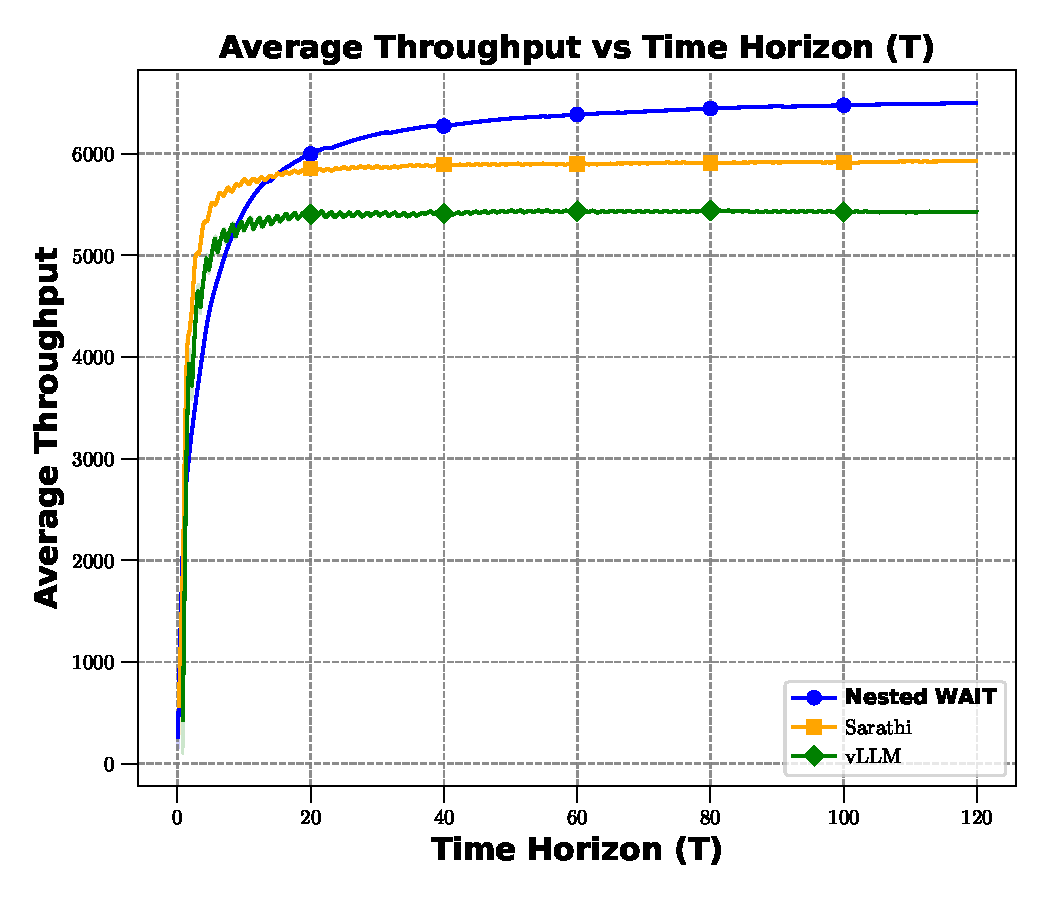
\includegraphics[width=\textwidth]{figures/test32_throughput.pdf}
    \\ \small{(a) Throughput (High QPS)}
\end{minipage}
\hfill
\begin{minipage}{0.45\columnwidth}
    \centering
    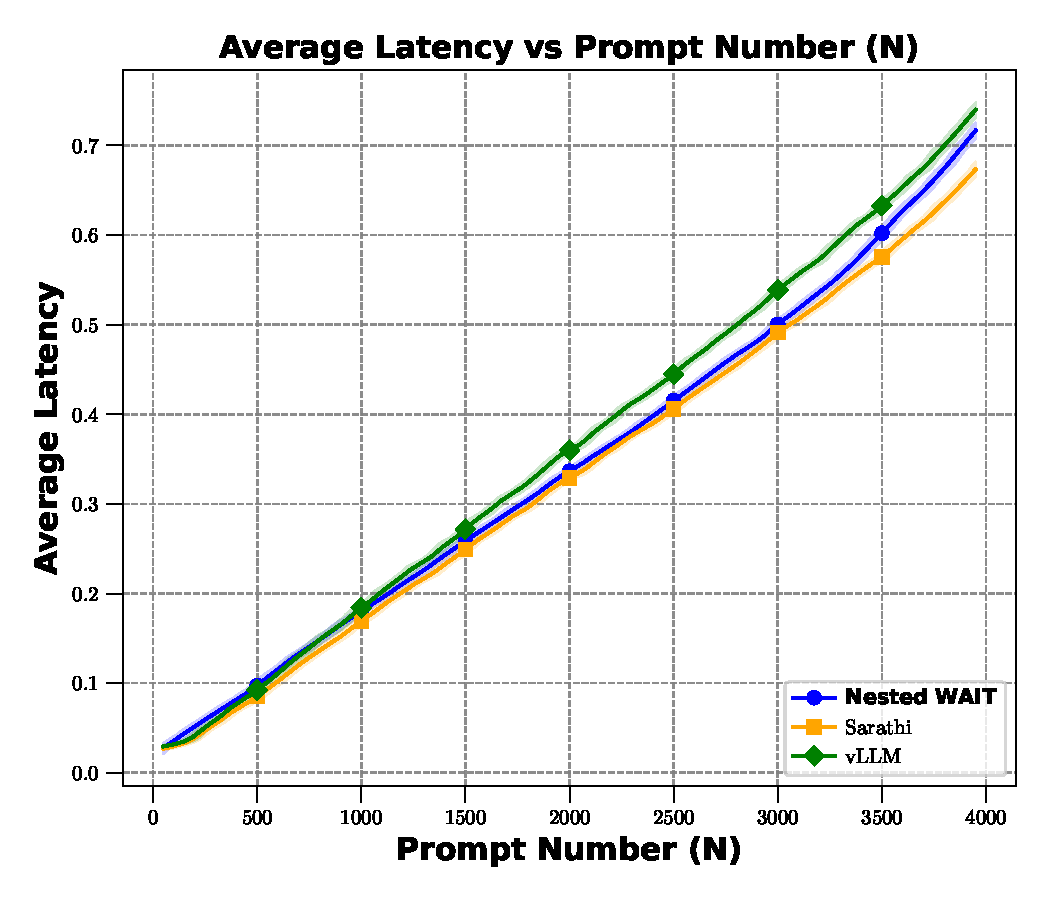
\includegraphics[width=\textwidth]{figures/test32_latency.pdf}
    \\ \small{(b) Latency (High QPS)}
\end{minipage}

\vspace{0.1cm}

% Row 2: Low QPS (55)
\begin{minipage}{0.45\columnwidth}
    \centering
    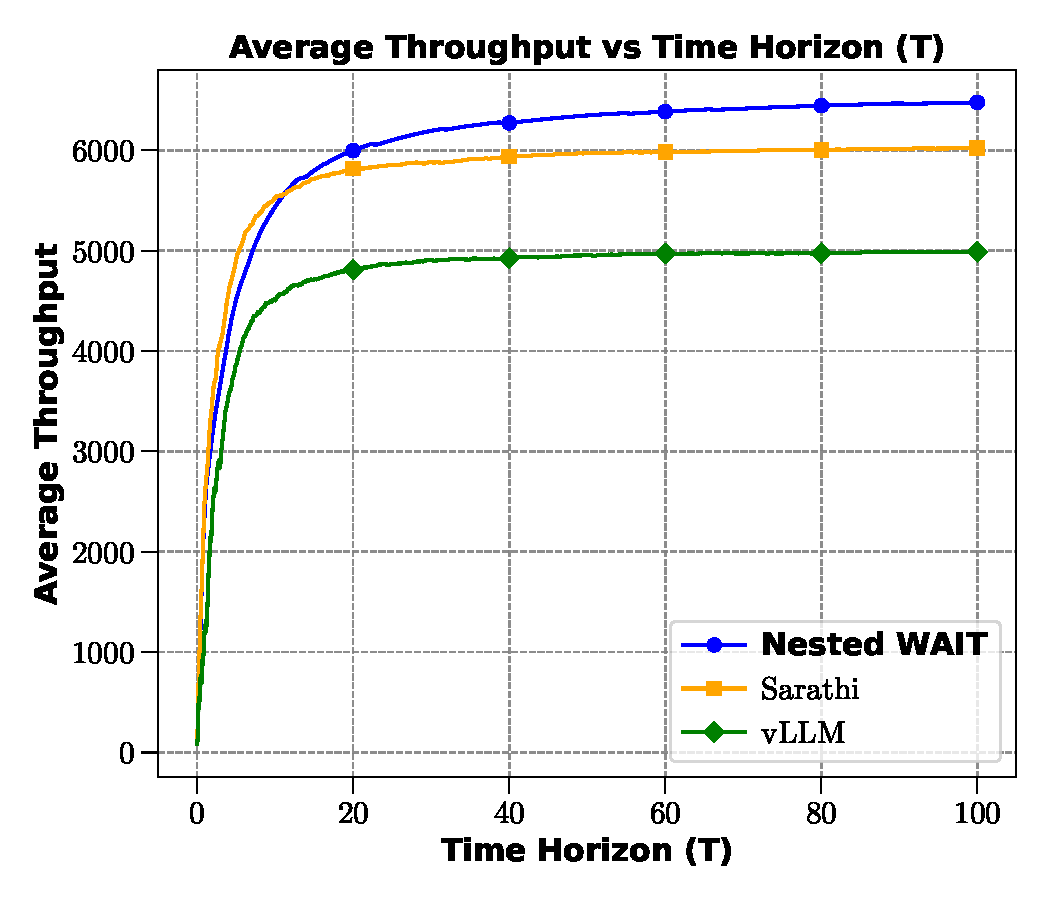
\includegraphics[width=\textwidth]{figures/test31_throughput.pdf}
    \\ \small{(c) Throughput (Low QPS)}
\end{minipage}
\hfill
\begin{minipage}{0.45\columnwidth}
    \centering
    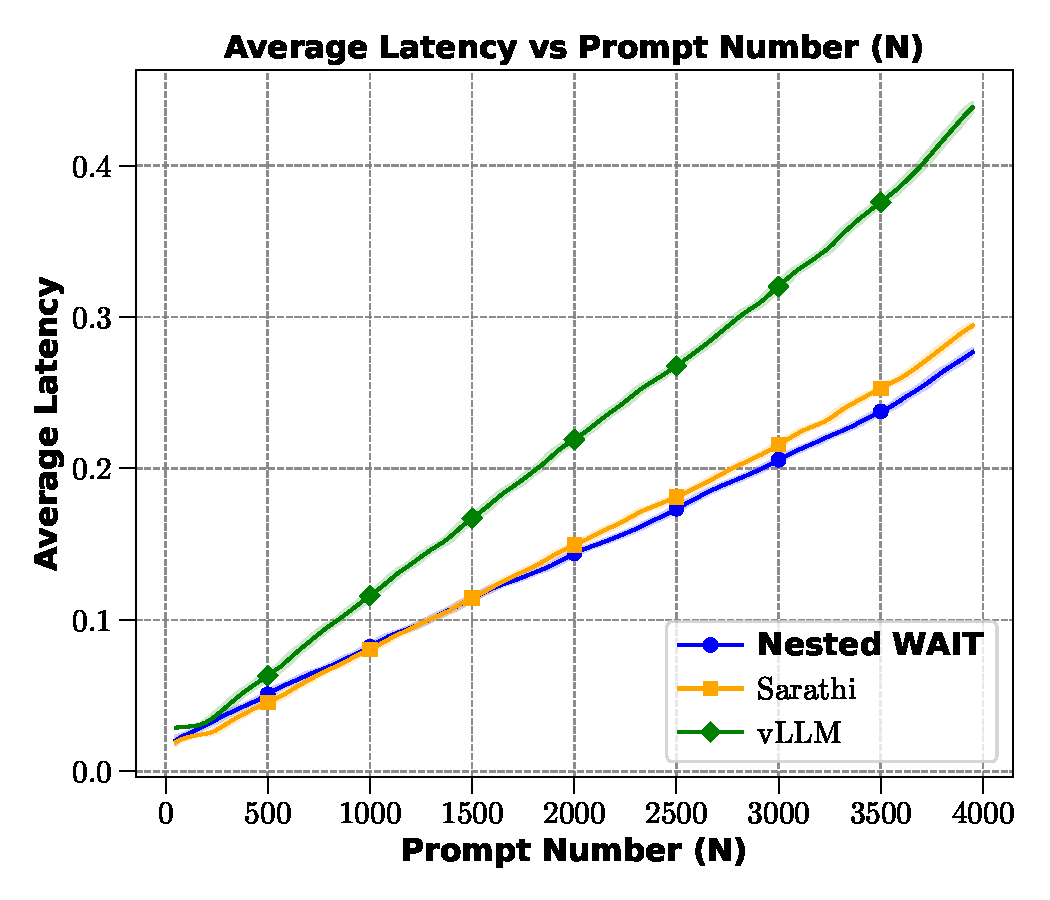
\includegraphics[width=\textwidth]{figures/test31_latency.pdf}
    \\ \small{(d) Latency (Low QPS)}
\end{minipage}

\caption{Performance on LMSYS-Chat-1M at 550 QPS (top) and 55 QPS (bottom). Nested WAIT improves throughput 12-25\% while maintaining competitive latency.}
\label{fig:performance_comparison}
\end{figure}


\section{Related Work and Conclusions}

\subsection{Related Work}

\textbf{Operations Research Perspective.} Recent works \cite{jaillet2025onlineschedulingllminference, wang2025llm, chen2025adaptively} analyze LLM scheduling from online algorithms viewpoint. Jaillet et al. assume constant $\tau = 1$, missing memory bandwidth effects. Our $\tau = d_0 + d_1 M$ model reveals how larger batches increase throughput but risk overflow—the core trade-off that drives eviction prevention. Li et al. \cite{li2025throughput} study general batch processing; our work focuses on memory-centric eviction prevention.

\textbf{System-Level LLM Inference.} vLLM \cite{kwon2023efficient} and Sarathi \cite{agrawal2023sarathi} use FCFS-based batching but lack eviction prevention mechanisms. DistServe \cite{zhong2024distserve} and Splitwise \cite{patel2024splitwise} implement Prefill-Decode disaggregation; our model applies directly to decode servers where the linear iteration time model holds exactly.

\textbf{Queueing Theory.} Fluid models \cite{mandelbaum1998strong, maglaras2000discrete} yield first-order approximations for stochastic systems. We adapt these techniques to LLM inference's unique challenges: dynamic memory growth, eviction feedback, and multi-stage processing.

\subsection{Conclusions}

We develop fluid-guided threshold-based algorithms for LLM inference scheduling under memory constraints. We contribute: (1) We model memory constraints by capturing dynamic KV cache growth. (2) We design eviction-prevention algorithms (WAIT and Nested WAIT) that achieve asymptotic optimality. (3) We validate these algorithms on real-world data, achieving 12-25\% throughput improvement.

Our data-driven framework bridges operations research theory and AI systems practice, providing actionable insights for LLM serving infrastructure. Performance metrics from real-world serving logs and GPU profiling inform scheduling decisions, demonstrating how OR methods—grounded in system data and analytics—optimize modern AI infrastructure.

\textbf{Future Work.} Extensions include multi-GPU settings, time-varying arrivals, and disaggregated memory systems.


% References
\bibliographystyle{ieeetr}
\bibliography{references_iise}

\end{document}
